\subsubsection{HasEnhancedByteBufferAccess}
\label{sec:uml:input:hasenhancedbytebufferaccess}

\lstinline|HasEnhancedByteBufferAccess| 这个接口提供了一个加强的 字节型的,缓冲式的读取方式。
一共提供了两个方法 \lstinline|releaseBuffer()| 和 \lstinline|read()|,分别用于释放和取得一个\lstinline|ByteBuffer|.

%% 类图
如下图 \ref{fig:HasEnhancedByteBufferAccess} 是 这个接口的 UML 类图。
\begin{figure}[h]
\centering
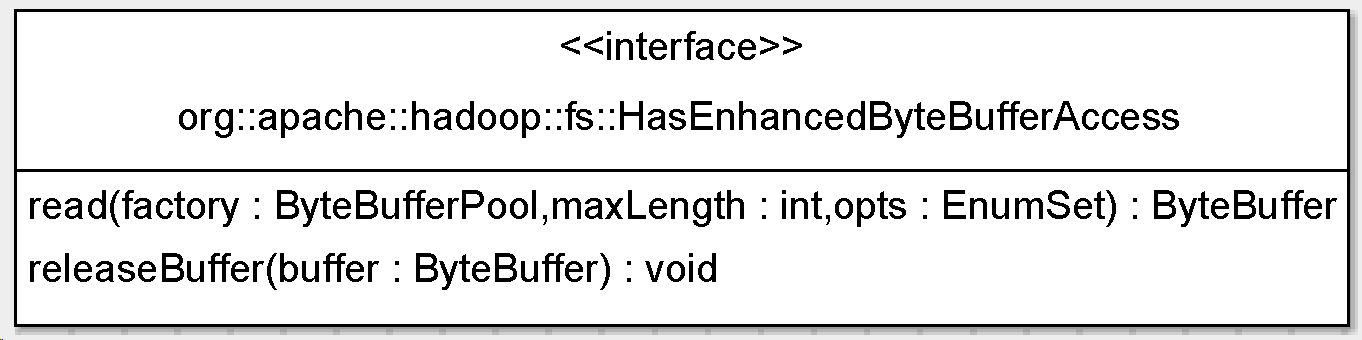
\includegraphics[width=1\linewidth]{HasEnhancedByteBufferAccess}
\caption{HasEnhancedByteBufferAccess 接口的 UML 类图}
\label{fig:HasEnhancedByteBufferAccess}
\end{figure}

%% 代码
这个接口一共定义了两个方法的接口。用于读取一个字节缓冲区,从字节缓冲区池中,同时还有释放的方法。
\begin{java}
@InterfaceAudience.Private
@InterfaceStability.Evolving
public interface HasEnhancedByteBufferAccess {
    public ByteBuffer read(ByteBufferPool factory, int maxLength, EnumSet<ReadOption> opts) throws IOException, UnsupportedOperationException;
    public void releaseBuffer(ByteBuffer buffer);
}    
\end{java}